%
% $RCSfile: framework.tex,v $
%
% Copyright (c) 2001-2004. Christian Heller. All rights reserved.
%
% Permission is granted to copy, distribute and/or modify this document
% under the terms of the GNU Free Documentation License, Version 1.1
% or any later version published by the Free Software Foundation;
% with no Invariant Sections, with no Front-Cover Texts and with no Back-Cover
% Texts. A copy of the license is included in the section entitled
% "GNU Free Documentation License".
%
% http://www.cybop.net
% - Cybernetics Oriented Programming -
%
% http://www.resmedicinae.org
% - Information in Medicine -
%
% @author Christian Heller <christian.heller@tuxtax.de>
% @author Jens Bohl <info@jens-bohl.de>
%

\section{CYBOP}
\label{cybop_heading}

Section \ref{design_principles_heading} introduced essential design patterns
that represent the main structure of the CYBOP framework. Section
\ref{an_extended_component_lifecycle_heading} explained the Component Lifecycle
and section \ref{ontology_heading} the well-known idea of ontology. Now these
design principles and conceptual architectures will be combined to comprise
their advantages and to increase the demanded quality characteristics: high
flexibility and maintainability.\\
\emph{Structure by Hierarchy} -- this is the basic idea behind CYBOP. Extending
the concept of Hierarchical Model-View-Controller to whole software architectures,
CYBOP was designed to be the domain-independent backbone for information systems
of any kind. Originally designed for medical purposes, it should also be usable
for insurance, financial or any other standard applications in future.

\subsection{Class Item}
\label{class_item_heading}

As shown, tree-like structures can be realized by the Composite pattern. In
CYBOP, this pattern can be found simplified in class {\tt Item} (figure
\ref{class_item_figure}) which is super type of all other classes. References,
respectively relations to child elements are held within a hashmap. No attributes
were used except of this hashmap. Every element of the map can be accessed by a
special key value. So, no particular {\tt get}- or {\tt set}-methods were needed
for attributes.

\begin{figure}[ht]
    \begin{center}
       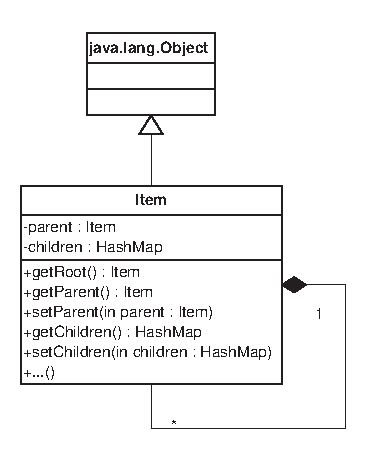
\includegraphics[scale=0.8]{eps/item.eps}
       \caption{Class Item}
       \label{class_item_figure}
    \end{center}
\end{figure}

\subsection{Basic Structure}
\label{basic_structure_heading}

Comprising the design patterns \emph{Composite}, \emph{Layers}, and
\emph{Chain of Responsibility}, the CYBOP framework is comparable to a big tree
containing objects organized in different levels. Figure \ref{basic_structure_figure}
shows the object tree and the different levels of granularity.

\begin{figure}[ht]
    \begin{center}
       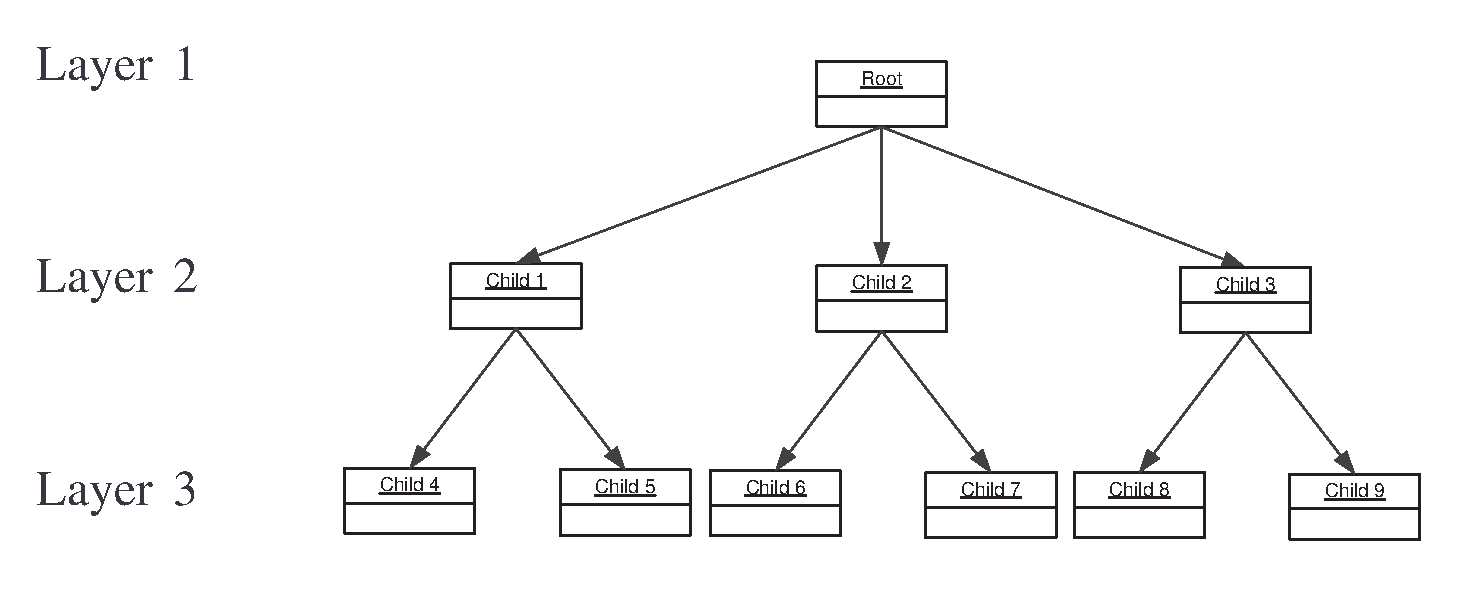
\includegraphics[scale=0.3]{eps/framework-structure.eps}
       \caption{Basic Structure}
       \label{basic_structure_figure}
    \end{center}
\end{figure}

